\documentclass[11pt]{article}

\usepackage[margin=1in]{geometry}
\usepackage{booktabs}
\usepackage{graphicx}
\usepackage{float}
\usepackage{hyperref}
\usepackage{longtable}
\usepackage{tabularx}
\usepackage{xcolor}

\graphicspath{{assets/puzzle-diagnostics/}}
\hypersetup{
  colorlinks=true,
  linkcolor=blue,
  urlcolor=blue
}

\title{Puzzle JEPA Diagnostic Report}
\author{sequence-editing puzzle pivot}
\date{2026-05-28}

\begin{document}
\maketitle

\section{Executive Summary}

The current puzzle JEPA scaffold is operational, but the first 5M-parameter
checkpoints are not yet solver-ready. Grid 0 and Grid 1 finished without OOMs or
Slurm failures. All Grid 1 H=1/2/4 planning solve rates are 0.0. Corrected Grid
1 diagnostics completed as Slurm array \texttt{3667044\_[0-4]} with exit
\texttt{0:0} for all tasks.

The main diagnostic result is clean and actionable: true re-encoded oracle
trajectories move monotonically toward the goal latent, while predicted latent
rollouts drift far from the true state and from the goal. The learned encoder
appears to represent progress, but the predictor does not compose over many
steps. In the full mutable action space, local oracle-action ranking is also
weak. Terminal LeWM-style reranking currently has no chance to help because the
bounded beam reaches no terminal boards or paths.

The immediate recommendation is not to run a size ablation yet. The next
eval-only diagnostic should compare pure latent rollout against symbolic
transition plus re-encoding after each planned step. If re-encoding recovers
planning, rollout drift is the blocker. If re-encoding does not recover
planning, the scorer/action-ranking objective is the blocker.

\section{Experiment Inventory}

\begin{table}[H]
\centering
\small
\begin{tabularx}{\textwidth}{l l l X}
\toprule
Job & Status & Runs & Notes \\
\midrule
\texttt{3664581\_[0-1]} & completed & Grid 0 Sudoku/Maze smoke &
Pipeline proof. Both runs wrote metrics and checkpoints. No OOMs. \\
\texttt{3665018\_[0-4]} & completed & Grid 1 5M curriculum &
Sudoku oracle, Sudoku 70/30, Sudoku 50/50, Maze oracle, Maze 70/30.
All H=1/2/4 solve rates were 0.0. \\
\texttt{3666870\_[0-4]} & completed & preliminary diagnostics &
Useful first drift signal, but Sudoku rank/planning used the old fill-only
action space, so corrected diagnostics supersede those rank/planner traces. \\
\texttt{3667044\_[0-4]} & completed & corrected diagnostics &
Final diagnostic set. Uses clue-mask mutable Sudoku actions, latent unrolls,
terminal-energy beam diagnostics, and latent-energy plots. \\
\bottomrule
\end{tabularx}
\caption{Puzzle JEPA jobs relevant to this report.}
\end{table}

\section{Model And Diagnostic Setup}

The JEPA model is decoder-free for these diagnostics. It encodes an objective
world state, conditions a latent predictor on an action, and compares the
predicted next latent to the encoded next state. For Sudoku, clues are immutable
and non-clue cells are mutable: they may be empty, overwritten, or temporarily
constraint-violating. For Maze, actions mark candidate empty cells as path cells.

The corrected diagnostics evaluate five questions:

\begin{enumerate}
  \item Does the model rank the oracle next action highly among legal actions?
  \item Does oracle-action latent rollout stay close to the true re-encoded
        state over 1, 2, 4, 10, 20, and terminal steps?
  \item Is latent MSE to the oracle goal monotonic along true oracle
        trajectories?
  \item Does bounded step-energy beam planning solve any examples?
  \item Does bounded terminal-energy reranking, closer to LeWM-style terminal
        scoring, improve over step-energy planning?
\end{enumerate}

Energy means mean squared error to the encoded oracle goal state. ``Predicted''
uses repeated latent prediction without re-encoding. ``True'' applies the same
oracle actions symbolically and re-encodes the resulting board/path state.

\section{Grid 1 Training Results}

\begin{table}[H]
\centering
\small
\begin{tabular}{lrrrrrrr}
\toprule
Run & Train & Eval & Top1 & Mean rank & H1 & H2 & H4 \\
\midrule
\texttt{sudoku\_oracle} & 0.0084 & 0.0085 & 0.0625 & 36.50 & 0.0 & 0.0 & 0.0 \\
\texttt{sudoku\_mix70\_30} & 0.0090 & 0.0084 & 0.0313 & 28.16 & 0.0 & 0.0 & 0.0 \\
\texttt{sudoku\_mix50\_50} & 0.0082 & 0.0074 & 0.0313 & 49.03 & 0.0 & 0.0 & 0.0 \\
\texttt{maze\_oracle} & 0.0020 & 0.0021 & 0.0000 & 16.00 & 0.0 & 0.0 & 0.0 \\
\texttt{maze\_mix70\_30} & 0.0022 & 0.0019 & 0.0000 & 245.50 & 0.0 & 0.0 & 0.0 \\
\bottomrule
\end{tabular}
\caption{Final Grid 1 training/evaluation metrics from \texttt{3665018\_[0-4]}.}
\end{table}

These losses show that one-step latent prediction is learnable, but they do not
translate into planner solves. In particular, lower one-step MSE does not
predict better action ranking or planning.

\section{Corrected Diagnostic Results}

\subsection{Aggregate Metrics}

\begin{table}[H]
\centering
\small
\begin{tabular}{lrrrrrr}
\toprule
Run & Top1 & Top5 & Mean rank & Pred. mono & True mono & Terminal pred. MSE \\
\midrule
\texttt{sudoku\_oracle} & 0.0088 & 0.0303 & 184.79 & 0.334 & 1.000 & 1.753 \\
\texttt{sudoku\_mix70\_30} & 0.0127 & 0.0420 & 182.01 & 0.352 & 0.999 & 1.729 \\
\texttt{sudoku\_mix50\_50} & 0.0127 & 0.0361 & 167.68 & 0.287 & 1.000 & 1.710 \\
\texttt{maze\_oracle} & 0.0078 & 0.0781 & 124.12 & 0.372 & 1.000 & 1.938 \\
\texttt{maze\_mix70\_30} & 0.0195 & 0.0391 & 205.27 & 0.436 & 1.000 & 1.956 \\
\bottomrule
\end{tabular}
\caption{Corrected diagnostics from \texttt{3667044\_[0-4]}. ``Pred. mono'' is the monotonicity rate of predicted latent energy to the goal under oracle-action latent rollout. ``True mono'' is the same measurement after symbolic transition and re-encoding.}
\end{table}

\subsection{Action Rank By Trajectory Depth}

\begin{table}[H]
\centering
\scriptsize
\begin{tabular}{lrrrr}
\toprule
Run & Depth 0.00 & Depth 0.25 & Depth 0.50 & Depth 0.75 \\
\midrule
\texttt{sudoku\_oracle} & 246.04 / 0.0039 & 213.61 / 0.0039 & 182.69 / 0.0078 & 96.85 / 0.0195 \\
\texttt{sudoku\_mix70\_30} & 243.80 / 0.0078 & 212.03 / 0.0000 & 157.51 / 0.0039 & 114.70 / 0.0391 \\
\texttt{sudoku\_mix50\_50} & 218.74 / 0.0000 & 202.12 / 0.0078 & 151.29 / 0.0156 & 98.56 / 0.0273 \\
\texttt{maze\_oracle} & 195.17 / 0.0000 & 145.11 / 0.0156 & 112.30 / 0.0000 & 43.92 / 0.0156 \\
\texttt{maze\_mix70\_30} & 276.73 / 0.0156 & 253.55 / 0.0000 & 186.17 / 0.0313 & 104.63 / 0.0313 \\
\bottomrule
\end{tabular}
\caption{Mean oracle-action rank / top1 by depth fraction. Ranking improves late in trajectories, but early decisions are poor, exactly where planning needs reliable guidance.}
\end{table}

\subsection{Planning Diagnostics}

\begin{table}[H]
\centering
\small
\begin{tabular}{lrrrrr}
\toprule
Run & Mode & Solves & Terminal rate & Mean steps & Mean remaining Hamming \\
\midrule
\texttt{sudoku\_oracle} & step / terminal & 0.0 / 0.0 & 0.0 / 0.0 & 55.13 & 52.50 \\
\texttt{sudoku\_mix70\_30} & step / terminal & 0.0 / 0.0 & 0.0 / 0.0 & 55.50 & 51.88 \\
\texttt{sudoku\_mix50\_50} & step / terminal & 0.0 / 0.0 & 0.0 / 0.0 & 54.63 & 51.75 \\
\texttt{maze\_oracle} & step / terminal & 0.0 / 0.0 & 0.0 / 0.0 & 109.50 & 36.00 \\
\texttt{maze\_mix70\_30} & step / terminal & 0.0 / 0.0 & 0.0 / 0.0 & 110.50 & 100.00 \\
\bottomrule
\end{tabular}
\caption{Bounded beam planning metrics. Step-energy and terminal-energy results match because the bounded beam reached no terminal candidates, so terminal reranking never got a useful candidate set.}
\end{table}

\section{Latent Energy Figures}

\begin{figure}[H]
\centering
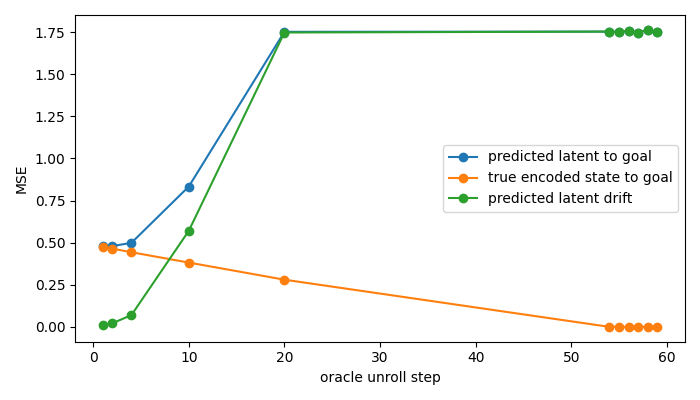
\includegraphics[width=0.88\textwidth]{sudoku-oracle-latent-energy-mse.png}
\caption{Sudoku oracle diagnostics. True re-encoded energy decreases toward zero; predicted rollout energy rises and drifts.}
\end{figure}

\begin{figure}[H]
\centering
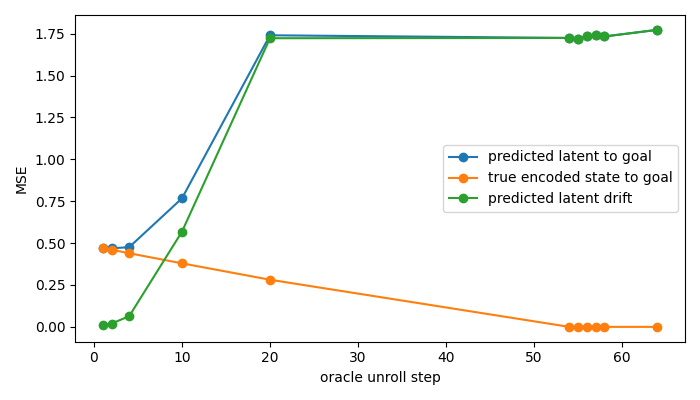
\includegraphics[width=0.88\textwidth]{sudoku-mix70-30-latent-energy-mse.png}
\caption{Sudoku 70/30 mutable-data diagnostics. The same qualitative pattern holds: re-encoded states are monotonic, predicted latents are not.}
\end{figure}

\begin{figure}[H]
\centering
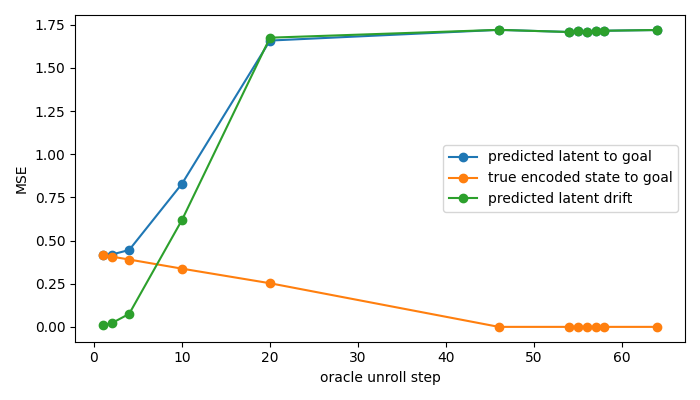
\includegraphics[width=0.88\textwidth]{sudoku-mix50-50-latent-energy-mse.png}
\caption{Sudoku 50/50 mutable-data diagnostics. This run has the best mean rank among Sudoku diagnostics, but still has non-compositional latent rollout.}
\end{figure}

\begin{figure}[H]
\centering
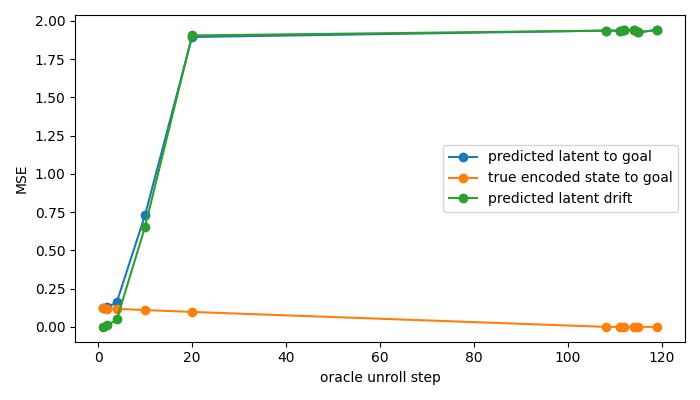
\includegraphics[width=0.88\textwidth]{maze-oracle-latent-energy-mse.png}
\caption{Maze oracle diagnostics. True path-state encodings approach the goal, but latent rollout diverges by 20 steps and remains far from the terminal goal.}
\end{figure}

\begin{figure}[H]
\centering
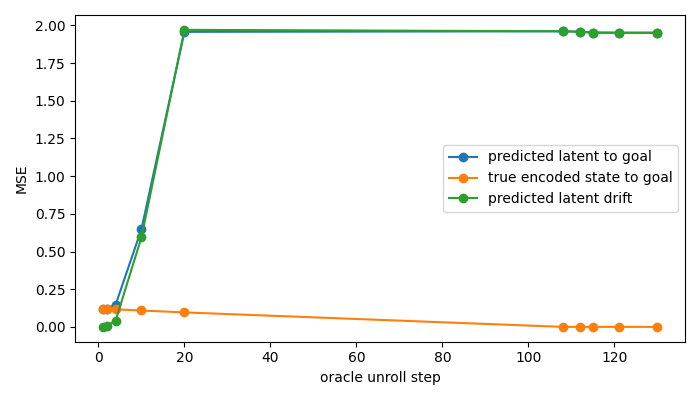
\includegraphics[width=0.88\textwidth]{maze-mix70-30-latent-energy-mse.png}
\caption{Maze 70/30 diagnostics. Off-path random marks do not fix the rollout or planning problem under the current scorer.}
\end{figure}

\section{Concrete Diagnostic Examples}

\subsection{Single Oracle Rollout Drift Examples}

\begin{table}[H]
\centering
\small
\begin{tabular}{lrrrr}
\toprule
Example & Step & Pred. goal MSE & True goal MSE & Latent drift MSE \\
\midrule
Sudoku oracle, example 0 & 1 & 0.4880 & 0.4879 & 0.0076 \\
Sudoku oracle, example 0 & 2 & 0.4906 & 0.4808 & 0.0197 \\
Sudoku oracle, example 0 & 4 & 0.5119 & 0.4613 & 0.0702 \\
Sudoku oracle, example 0 & 10 & 0.8337 & 0.3978 & 0.5715 \\
Sudoku oracle, example 0 & 20 & 1.7530 & 0.2817 & 1.7500 \\
Sudoku oracle, example 0 & terminal 56 & 1.7434 & 0.0000 & 1.7434 \\
\midrule
Maze oracle, example 0 & 1 & 0.1234 & 0.1213 & 0.0022 \\
Maze oracle, example 0 & 2 & 0.1288 & 0.1197 & 0.0099 \\
Maze oracle, example 0 & 4 & 0.1654 & 0.1170 & 0.0523 \\
Maze oracle, example 0 & 10 & 0.8069 & 0.1090 & 0.7355 \\
Maze oracle, example 0 & 20 & 1.9034 & 0.0952 & 1.9074 \\
Maze oracle, example 0 & terminal 111 & 1.9362 & 0.0000 & 1.9362 \\
\bottomrule
\end{tabular}
\caption{Concrete drift records from \texttt{drift\_records.jsonl}. The true encoded state monotonically approaches the goal; latent rollout quickly stops tracking it.}
\end{table}

\subsection{Representative Planner Trace Prefixes}

Each trace below shows the first four actions chosen by the planner and the
corresponding oracle next actions. Coordinates are \texttt{(row, col, value)}.
The value is a Sudoku digit for Sudoku and path token 4 for Maze.

\begin{longtable}{lrrrrp{0.25\textwidth}p{0.25\textwidth}}
\caption{Representative planner traces from \texttt{diagnostics.json}. The planner often locks into wrong cells or oscillates on mutable Sudoku cells.}\\
\toprule
Run & Solved & Steps & Remaining & Ranks & Chosen first four & Oracle first four \\
\midrule
\endhead
\texttt{sudoku\_oracle} & no & 12 & 53 & 36, 334, 219, 272 &
(6,0,2), (8,1,6), (3,2,1), (6,1,2) &
(6,0,5), (0,6,8), (6,3,8), (4,0,8) \\
\texttt{sudoku\_mix70\_30} & no & 12 & 52 & 434, 336, 301, 379 &
(8,5,2), (8,4,2), (5,2,2), (3,5,3) &
(5,7,1), (5,8,6), (7,7,8), (4,1,1) \\
\texttt{sudoku\_mix50\_50} & no & 12 & 56 & 45, 375, 142, 377 &
(6,0,7), (6,7,7), (6,0,6), (6,0,7) &
(6,7,3), (8,0,5), (1,3,5), (8,2,7) \\
\texttt{maze\_oracle} & no & 12 & 109 & 33, 3, 267, 36 &
(3,5,4), (22,3,4), (11,14,4), (7,17,4) &
(11,13,4), (11,14,4), (12,14,4), (13,14,4) \\
\texttt{maze\_mix70\_30} & no & 12 & 126 & 279, 254, 318, 539 &
(27,27,4), (16,15,4), (25,27,4), (0,27,4) &
(1,5,4), (1,4,4), (1,3,4), (1,2,4) \\
\bottomrule
\end{longtable}

\subsection{Trace Interpretation}

The Sudoku examples show the failure mode introduced by the correct mutable
action space. The model can choose any non-clue cell and any digit, including
overwrites and conflict-producing digits. This makes the legal action set about
450--500 actions. The oracle action is rarely top ranked early, and the planner
often chooses repeated writes to the same high-scoring cells rather than making
steady progress through the solution.

The Maze examples show a related but spatially clearer failure mode. The oracle
path is locally coherent, but the planner often marks distant cells because the
latent score does not sufficiently reward path-contiguous progress. Even when
the oracle action briefly ranks high, the next decisions often drift away from
the path.

\section{Interpretation}

\paragraph{What worked.}
The training and diagnostic infrastructure works. Checkpoints, metrics,
rank records, drift records, and figures are produced reliably. One-step losses
are low, and the encoder's true re-encoded states carry a strong progress signal
to the oracle goal.

\paragraph{What failed.}
The predictor is not a reliable multi-step world model yet. Under oracle
actions, predicted latents drift from true re-encoded latents within 10--20
steps. By terminal oracle states, predicted latents remain roughly 1.7--2.0 MSE
from the goal. Planning also fails before terminal scoring can matter because
the bounded beam does not reach terminal candidates.

\paragraph{Most likely bottleneck.}
The bottleneck is currently latent rollout drift plus weak early action ranking,
not raw model capacity. A larger model may reduce loss, but the diagnostics do
not yet show a 5M model with a usable planning signal.

\section{Next Steps}

\begin{enumerate}
  \item Run an eval-only Grid 3 slice comparing latent-only rollout with
        symbolic transition plus re-encoding after each step.
  \item If re-encoding recovers planning, train the predictor with stronger
        multi-step rollout repair or truncated unroll losses.
  \item If re-encoding does not recover planning, add a learned value, verifier,
        or contrastive energy objective rather than increasing model size first.
  \item For the next training grid, remove task-id conditioning and the selected
        cell marker. We train one model per task, and the action already carries
        row, column, and value.
  \item Only submit 10M/20M size ablations once at least one 5M checkpoint shows
        a nonzero final planning signal or a fixed diagnostic exposes a concrete
        evaluation bug.
\end{enumerate}

\section{Artifact Index}

Primary outputs used by this report:

\begin{itemize}
  \item \texttt{/home/vault/c107fa/c107fa12/sequence-editing/runs/*/diagnostics/diagnostics.json}
  \item \texttt{/home/vault/c107fa/c107fa12/sequence-editing/runs/*/diagnostics/rank\_records.jsonl}
  \item \texttt{/home/vault/c107fa/c107fa12/sequence-editing/runs/*/diagnostics/drift\_records.jsonl}
  \item \texttt{docs/assets/puzzle\_diagnostics/*\_latent\_energy\_mse.png}
\end{itemize}

\end{document}
